\section{Observed-quote and touch-price sensitivity}

The licensed-quote audit changes only spread evidence. It preserves positions, gross
holding-period returns, non-spread costs, integer decisions, and survival gates. The mid
scenario uses observed
midpoints while retaining the stated non-spread terms. The touch scenario substitutes
observed entry and exit spreads. The worst scenario uses the entry-window maximum spread
and the observed exit spread.

Months without observed quotes keep the modeled cost. The audit counts these gaps rather
than fabricating a quote. Reconstructing modeled cost from the recorded components leaves a
maximum absolute gap below \(10^{-16}\). The scenario ladder therefore isolates the effect
of quote-based spread evidence.

\begin{figure}[!ht]
\centering
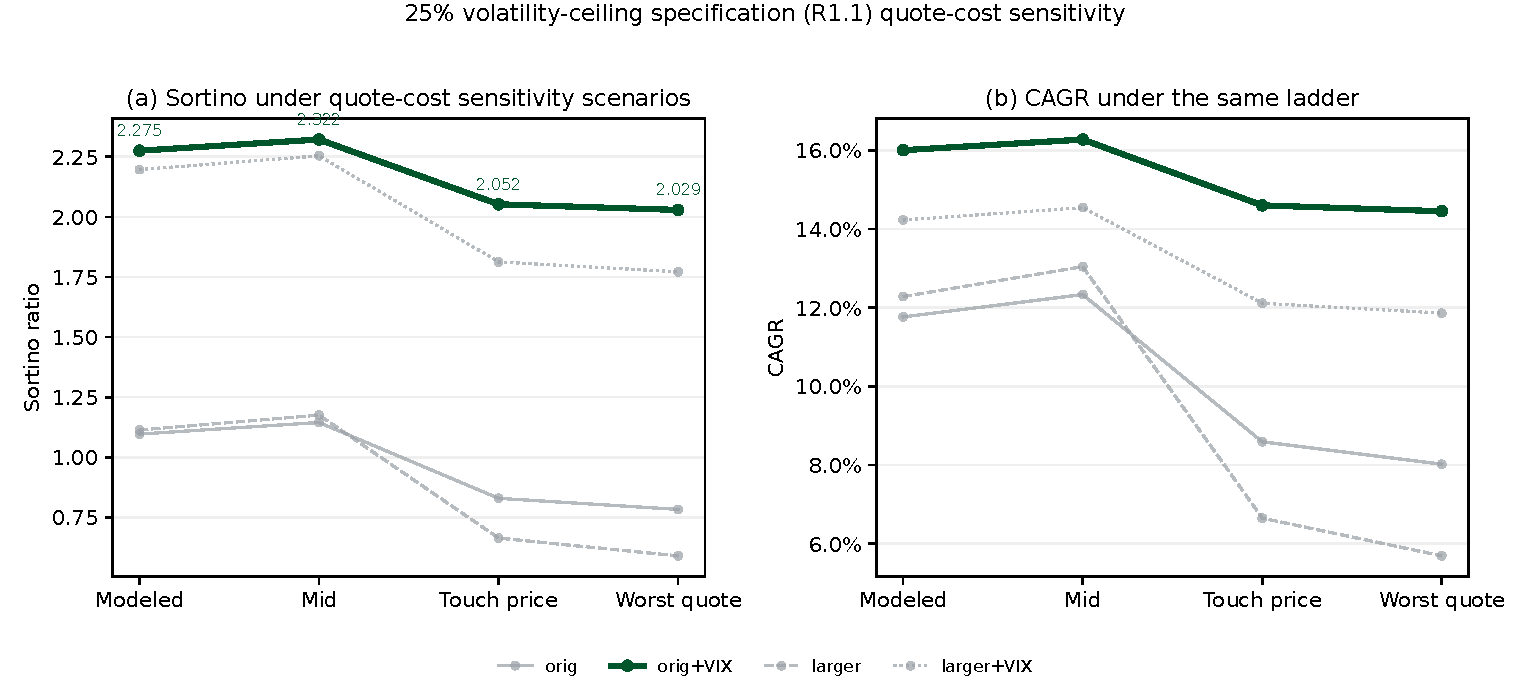
\includegraphics[width=0.95\textwidth]{figures/short_audit_scenario_ladder.pdf}
\caption{Quote-cost sensitivity for R1.1. The x axis moves from modeled costs
through midpoint, touch-price, and worst-quote scenarios. The eight-name plus VIX
configuration uses the heavier line.}
\label{fig:audit_ladder}
\end{figure}

Figure~\ref{fig:audit_ladder} shows a small improvement at midpoint and lower results in
the touch-price and worst-quote scenarios. The eight-name plus VIX R1.1 path does not
reach zero wealth in these sensitivities. These are cost sensitivities on fixed
positions, not realized execution records or backtests selected from the quote sample.

\subsection{Headline configuration}

The spread-source distinction decides which historical result deserves emphasis.
Broad-name and VIX rows lack exact panel CBBO in the historical cost stack, so those rows use
the inferred proxy. The licensed audit finds wider observed broad-name spreads than the
proxy assumed. Figure~\ref{fig:proxy_coverage} places proxy reliance, observed-quote
coverage, and spread quantiles in one view.

\begin{figure}[!ht]
\centering
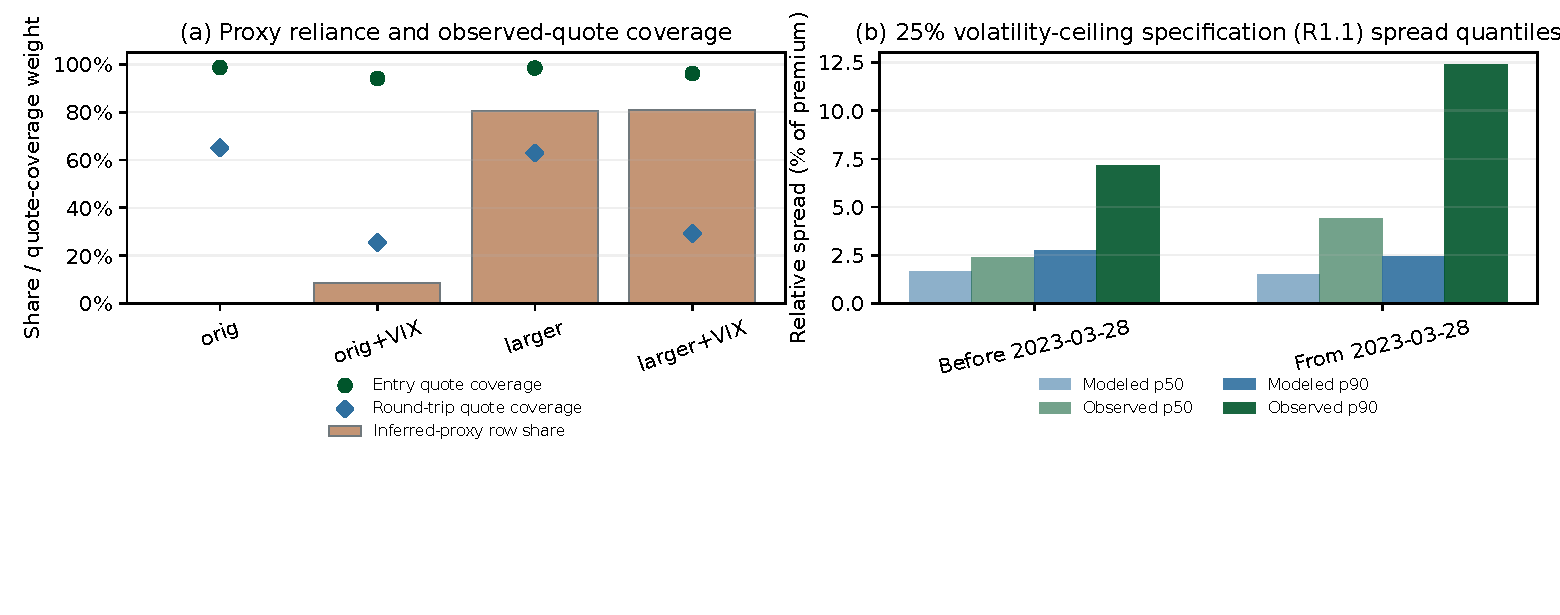
\includegraphics[width=0.97\textwidth]{figures/short_proxy_coverage_evidence.pdf}
\caption{Proxy reliance and licensed-quote evidence. Panel (a) compares inferred-proxy
row share with absolute-weighted entry and round-trip quote coverage. Panel (b) pools
R1.1 positions across configurations and compares modeled and observed spread quantiles
before and after the quote-schema cutover.}
\label{fig:proxy_coverage}
\end{figure}

For the 56-name plus VIX configuration, touch-price Sortino falls from 2.197 to 1.812, a
17.5 percent decline; entry and round-trip coverage are 96.2 and 29.1 percent. For the
eight-name plus VIX configuration, it falls from 2.275 to 2.052, a 9.8 percent decline;
entry and round-trip coverage are 94.1 and 25.5 percent. The eight-name plus VIX result is
reported because its equity-option spread evidence is exact in the historical panel and its
touch-price path does not reach zero wealth. Low round-trip coverage
limits the execution interpretation. Appendix~\ref{app:audit_tables} reports the full
scenario, spread, and liquidity tables.

\FloatBarrier
\section{Robustness, capacity, and limitations}

The validation suite separates path fragility from formal inference. CPCV recombines
purged test blocks and preserves the zero-wealth boundary.

Monte Carlo resampling tests return ordering. Refit and reprice exercises repeat
estimation and option repricing under locked cost rules. These simulations are path-risk
diagnostics, not tradable histories or confirmatory observations.

\begin{figure}[!ht]
\centering
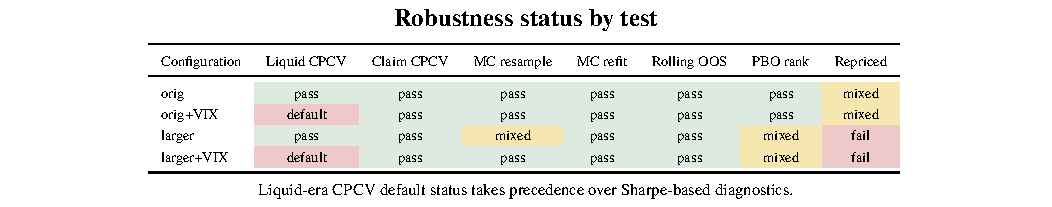
\includegraphics[width=0.94\textwidth]{figures/short_robustness_heatmap.pdf}
\caption{Robustness status for the four E1 universes. Liquid-era CPCV marks the
VIX-enabled configurations as defaulted because their paths reach zero. Claim-window
and simulation results do not override that outcome.}
\label{fig:short_robustness}
\end{figure}

The VIX-enabled E1 configurations have a CPCV default share of 1.000. Once wealth reaches
zero, their Sharpe quantiles are not meaningful; the corrected evidence reports them as
NA and assigns \texttt{fail\_default}. Sharpe and Sortino ratios follow
\citet{sharpe1966} and \citet{sortino_price1994}. In the liquid-era scope, full-cost net
PBO is 0.1795 within the eight-name plus VIX configuration and 0.3846 when all
configurations are ranked together. In the narrower post-2020 claim window, the
corresponding estimates are 0.0000 and 0.4487. The scopes answer different ranking
questions, and neither covers the complete research history. The incomplete R1 and R1.1
registries record lower bounds of 598 and 607 known trials.

\begin{table}[H]
\centering
\caption{Formal inference for the static full-cost net prototype books over the common
test window. The table reports uncertainty, probabilistic and deflated Sharpe measures,
and comparisons with stock and capped naive baselines.}
\label{tab:short_inference_panel}
\resizebox{\textwidth}{!}{\begin{tabular}{lrrrrrrrrr}
\toprule
Config & Net Sharpe & CI lo & CI hi & PSR & DSR & dSR stock & p stock & dSR naive & p naive \\
\midrule
orig & 0.778 & 0.163 & 1.433 & 0.973 & 0.945 & -0.131 & 0.776 & 0.413 & 0.014 \\
orig+VIX & 1.383 & 0.895 & 1.971 & 1.000 & 0.997 & 0.474 & 0.383 & 2.273 & 0.000 \\
larger & 0.587 & 0.029 & 1.173 & 0.925 & 0.745 & -0.322 & 0.436 & -0.009 & 0.967 \\
larger+VIX & 1.628 & 1.111 & 2.245 & 1.000 & 0.996 & 0.719 & 0.179 & 1.335 & 0.000 \\
\bottomrule
\end{tabular}
}
\end{table}

Rolling out-of-sample tests retrain only on earlier observations. The common ledger keeps
the comparison dates fixed across universes. Table~\ref{tab:short_inference_panel} shows
that multiple-testing adjustment weakens the interpretation of the static prototype
results but does not erase every signal. The survival failure still dominates the
prototype's attractive later-window statistics.

\FloatBarrier
\subsection{Capacity and execution limits}

Figure~\ref{fig:capacity_spreads} compares deployed gross with the sum of contract
liquidity caps and records the spread-source mix. The \(\$1\) million cap budget is a
local diagnostic and does not justify extrapolation to \(\$5\) million NAV.

\begin{figure}[H]
\centering
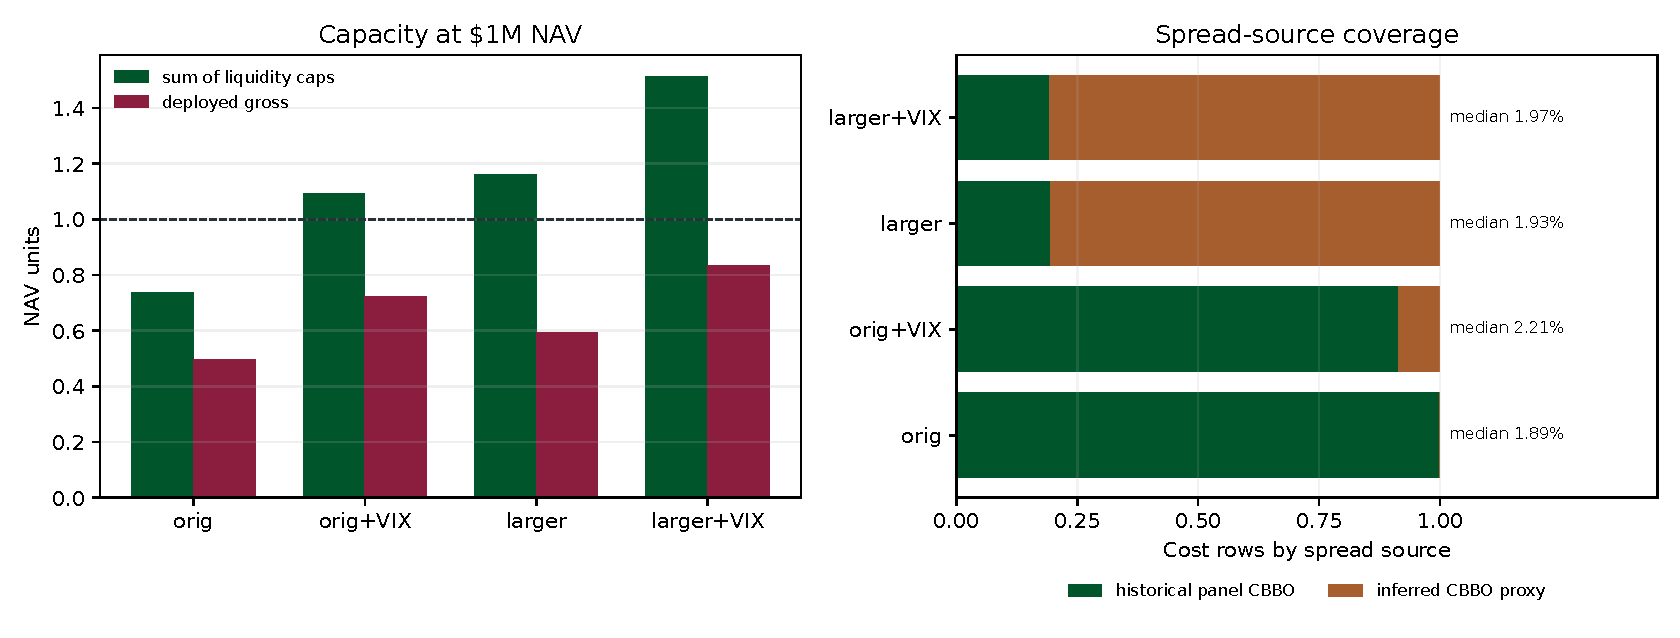
\includegraphics[width=0.94\textwidth]{figures/short_capacity_spread_panel.pdf}
\caption{Capacity and spread-source evidence at the stated account size. Panel (a)
compares deployed gross with the sum of liquidity caps. Panel (b) shows exact panel CBBO
and inferred-proxy shares.}
\label{fig:capacity_spreads}
\end{figure}

Multi-exchange routing could change available depth, but the paper makes no claim about
routing improvement. The data contain no routed orders or realized executions. The allocator checks assignment
exposure before execution. Any whole-contract breach fails closed to cash. The VIX-40
risk-off arm also remains unscored without complete event quotes. A model price cannot
replace any of these missing observations after the fact.

The evidence supports one retrospective development candidate at the tested size and
under the documented source hierarchy. It does not support unrestricted capacity, live
execution quality, or performance outside the recorded universes.

\FloatBarrier
\section{Conclusion and prospective protocol}

The prospective protocol freezes code, configuration, source hashes, artifact hashes,
and the decision rule before the system scores a future observation. Confirmation requires 36
untouched monthly observations beginning 2026-07-31. A missing quote, failed integer
conversion, or survival breach keeps its original status in the ledger. No later return
can change that status.

E1 compounds rapidly in the later window but fails when its March 2020 CPCV paths reach
zero wealth. R1 and R1.1 admit cash, retain the complete covariance, and enforce the
stated survival limits. The eight-name plus VIX R1.1 path remains solvent in the
touch-price cost sensitivity. It is a retrospective candidate, not a confirmatory result.

\FloatBarrier
